\documentclass[a4paper,12pt,twoside]{report}
% Pakketten
\usepackage[dutch]{babel}
\usepackage[T1]{fontenc}
\usepackage[margin=2.5cm]{geometry}
\usepackage{amsmath}
\usepackage{graphicx}
\usepackage{booktabs}
\usepackage{hyperref}
\usepackage{enumitem}
\usepackage{microtype}
\usepackage{../../school-macros}
\begin{document}
% Titelinformatie
\kuleuventitle
{LaTeX Samenvatting}
{Information Management}
{Louic Cooreman}
{Academiejaar 2025-2026}
\tableofcontents
\newpage
\chapter{Inleiding}
\subsection*{Waarom hebben we dit vak als ingenieur?}
Als ingenieur moet je inzicht en vaardigheden verwerven in het omgaan met de opslag, het ophalen en de analyse van data. Moderne bedrijven eisen dergelijke kennis, omdat data steeds relevanter en belangrijker wordt.
\subsection{IT vs OT}
Vooraleer we starten is het belangrijk om het verschil te begrijpen tussen IT (Information Technology) en OT (Operational Technology). Wij als EM studenten zijn meer gefocust op OT, dit focust zich meer op de machines zelf en gaat over het beheren van de operatie van de fysische processen en de machines die dit dan uitvoeren. IT houdt zich bezig met informatie/data, het beheert de "flow" van data, dit is dus puur digitaal via netwerken. OT heeft echter ook wat data, sensoren geven data, wordt opgeslaan en actuatoren gebruiken deze.
\begin{figure}[H]
	\centering
	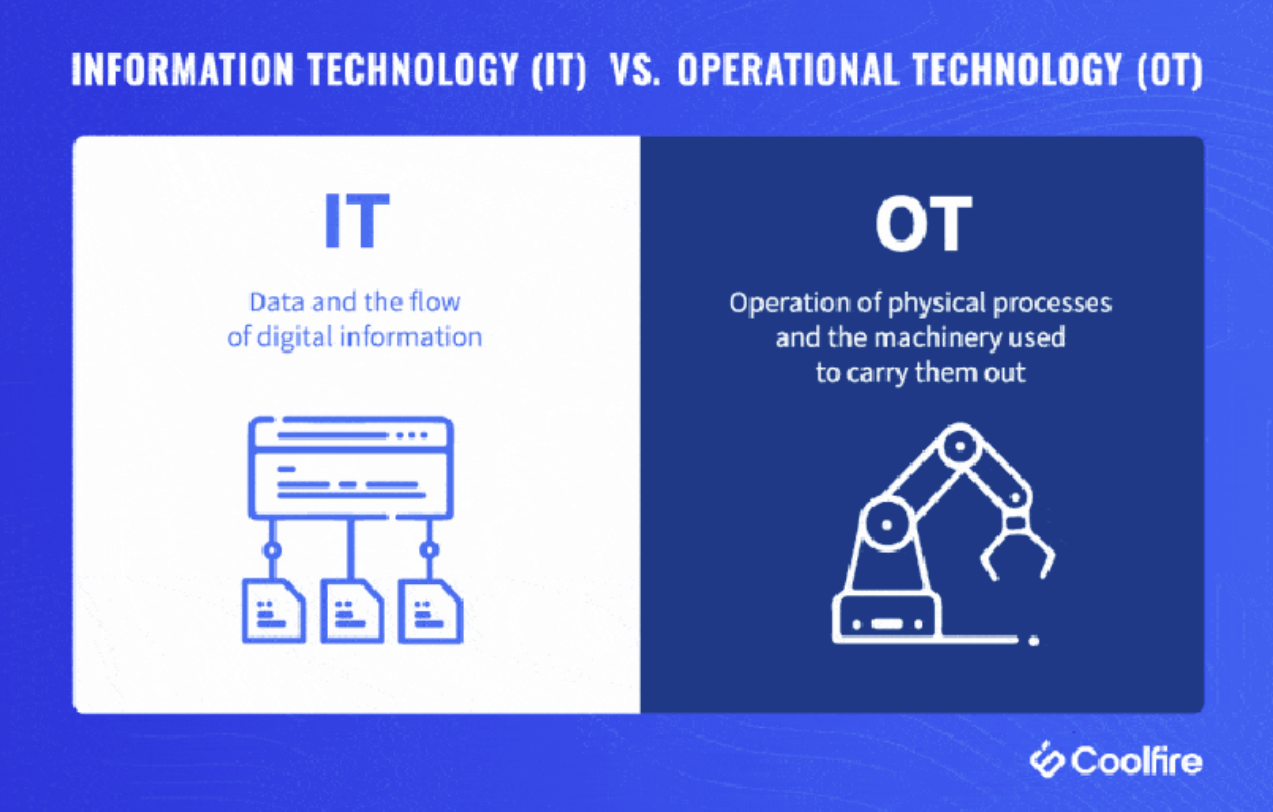
\includegraphics[width=0.6\textwidth]{IT_vs_OT.png}
	\caption{Information Technology (IT) vs Operational Technology (OT)}
\end{figure}
De proff zei in de les ook nog deze goofy zin : 
\begin{conceptbox}[Goofy quote]
\textbf{“You are milking the cow, but someone else is drinking the milk.”}
\end{conceptbox}
Uitleg : 
In OT bedien je de machines en genereer je de data, maar in IT gebruiken anderen die data om beslissingen te nemen en waarde te creëren.
\newline
\textbf{In deze cursus} gaan we ons eerst focussen op hoe computers informatie processen en storen. Later bekijken we dan ook hoe informatie uitgewisseld wordt tussen systemen en daarna kijken we hoe deze ideën uitgebreid worden en hoe informatie beschermd kan worden.
\newpage
\chapter{Les 1: De waarde van data}
\subsection{DIKW-piramide (Data, Information, Knowledge, Wisdom)}
De onderstaande figuur toont de DIKW-piramide, een klassiek model dat beschrijft hoe we ruwe feiten (data) omzetten in betekenisvolle inzichten (informatie), vervolgens in toepasbare kennis, en uiteindelijk in wijsheid.
De proff stelt de vraag over waar de grens tussen mens en robot zich bevind, want tegenwoordig met AI kunnen we al heel veel van de piramide automatiseren, maar er is nog steeds een grens waar menselijke wijsheid nodig is.
Het is duidelijk dat computers en machines zich vroeger zich tot de onderste lagen van de piramide bevonden (data en informatie) en mensen bovenaan bij wijsheid.
\begin{figure}[H]
    \centering
    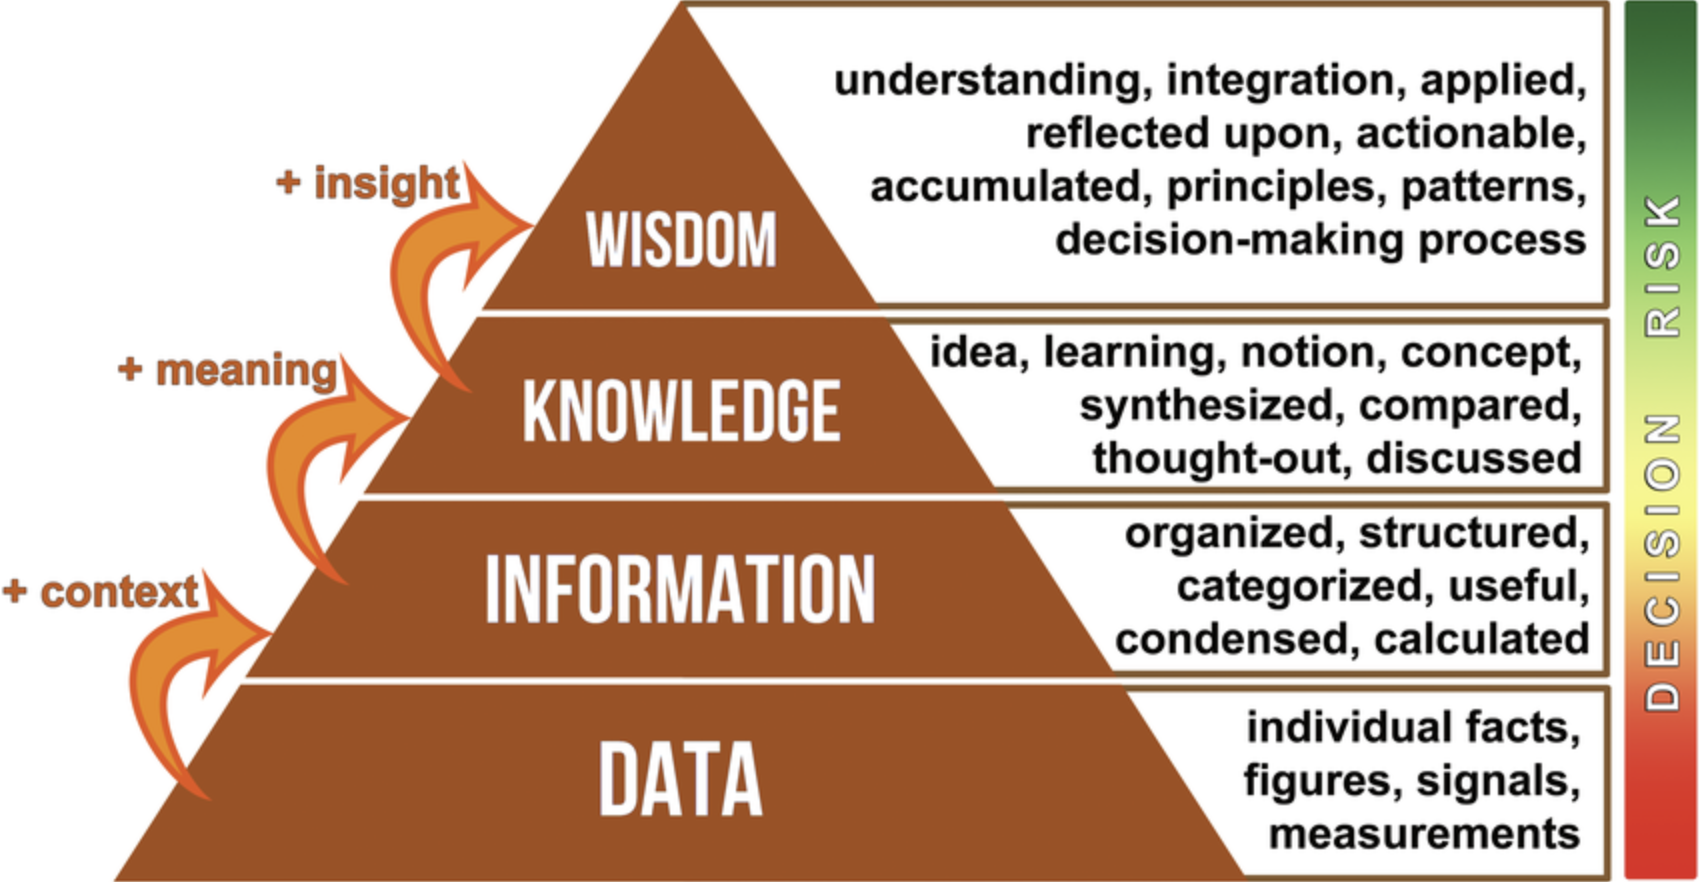
\includegraphics[width=0.6\textwidth]{DIKW.png}
    \caption{DIKW-piramide (Data, Information, Knowledge, Wisdom)}
\end{figure}
\newpage
\chapter{Les 2: De opkomst van computerarchitectuur, besturingssystemen en programmeren}
\subsection{Wat is een computer?}
Vroeger was een computer btw puur mechanisch met flip flops enzo, nu is dit natuurlijk al wat anders, dit was natuurlijk puur voor berekeningen.
\begin{conceptbox}[Definitie van een computer]
    Een computer is een machine dat:
    \begin{itemize}
        \item Een input kan ontvangen
        \item Data processed tot een set van instructies (een programma)
        \item Data/instructies kan opslaan (store)
        \item Een output kan genereren
    \end{itemize}
    Verschillende soorten computers voor verschillende doelen zijn dus mogelijk, bvb een standaard computer met windows, of een console, smartphone, server, ...
    Deze definitie is onafhankelijk van de grootte of technologie.
    \begin{figure}[H]
      \centering
      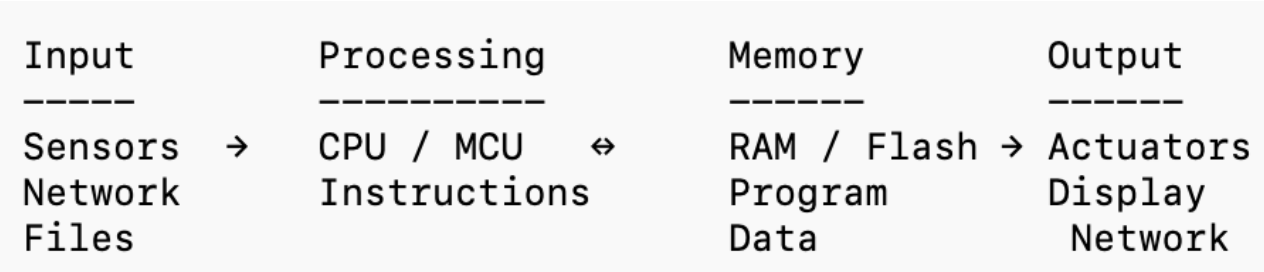
\includegraphics[width=0.8\textwidth]{cyclus_computer.png}
      \caption{Basis principe van computerarchitectuur (cyclus)}
      \label{}
     \end{figure}
\end{conceptbox}
Van zodra je de input hebt ga je een proces hiermee moeten doen, een soort van calculatie, typisch betekent dit een set van instructies lezen (programma), in code.
Vroeger zag dit er zo uit :
\begin{figure}[H]
  \centering
  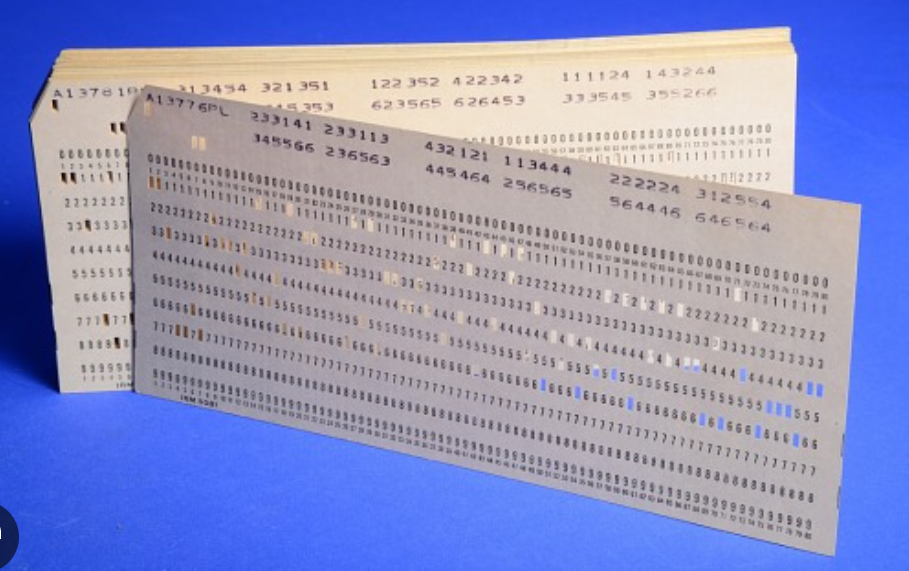
\includegraphics[width=0.4\textwidth]{punchcards.png}
  \caption{Punchcards}
  \label{fig:punchcards.png}
 \end{figure}
Nu is dit natuurlijk vereenvoudigd tot een programma dat je kan uitvoeren op je computer, maar het principe is hetzelfde, je hebt een programma dat instructies bevat die de computer moet uitvoeren.
Ze worden allemaal, op de een of andere manier, uitgevoerd door de hoofdcomputer en de hoofdprocessor, die de instructies op de gegevens toepast en vervolgens doorgaat naar de volgende instructies.
\newpage
Het belangrijkste onderdeel van de loop is de CPU (Central Processing Unit), dit is het onderdeel dat de beslissingen maakt.
\subsection{De CPU (Central Processing Unit)}
Dit vertaalt de beslissingen van je code (bvb C++) naar iets dichter bij de machine, dit is de assembly code, dit is een soort van taal die direct door de machine begrepen wordt, maar nog steeds leesbaar is voor mensen.
\newline
Nu gaan we een beetje kijken naar de architectuur van de CPU, we kunnen hier al 3 belangrijke onderdelen onderscheiden (we gaan het simpel houden):
\begin{itemize}
    \item \textbf{Arithmetic Logic Unit (ALU):} Voert de berekeningen uit, zoals optellen, aftrekken, vermenigvuldigen, delen, en logische operaties.
    \item \textbf{Control Unit (CU):} Deze eenheid wordt omschreven als het 'brein van het brein' of zoals de proff het zegt : 'De orchestra beheerder'. De CU is verantwoordelijk voor het coördineren en beheren van de prestaties van de gehele CPU. De belangrijkste taken zijn het ophalen, decoderen en uitvoeren van instructies, daarbij stuurt de CU aan welke circuits er werken en beheert het de toegang tot het geheugen, de veldbussen en gedeelde invoer/uitvoer-apparaten (zoals USB en SSD-schijven)
    \item \textbf{Main memory (Werkgeheugen):} Het geheugen werkt samen met de ALU en CU om instructies en resultaten op te slaan en aan te leveren.
\end{itemize}
De volgende figuur toont de controle loop (cyclus) in 4 stappen:
\begin{figure}[H]
  \centering
  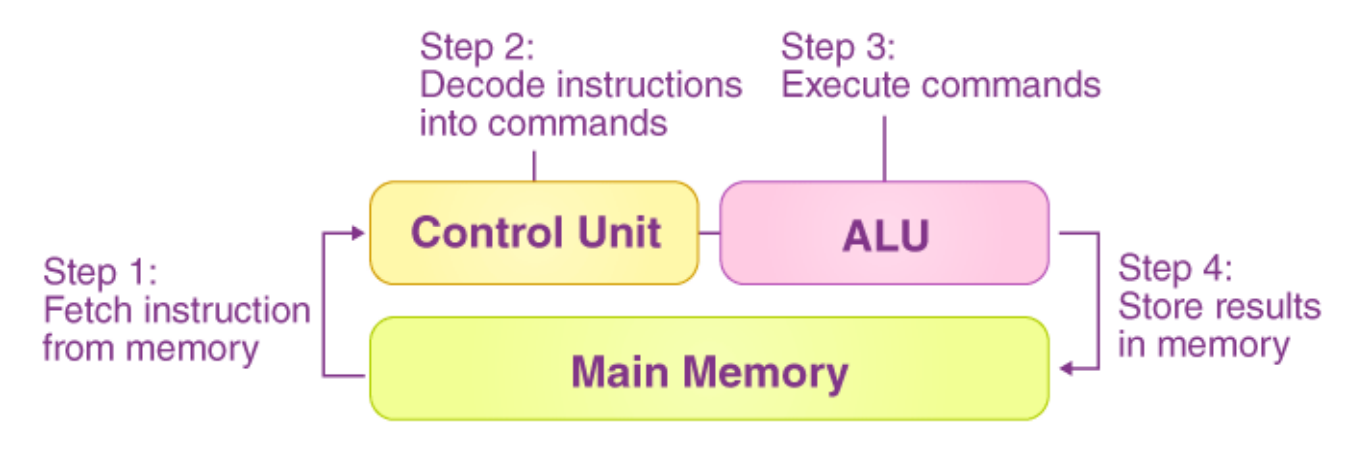
\includegraphics[width=0.8\textwidth]{CPU_controlloop.png}
  \caption{CPU architectuur}
  \label{fig:CPU_controlloop.png}
 \end{figure}
\subsection{Opslagen van instructies en data}
Dit is natuurlijk belangrijk voor de werking van een computer.
Terwijl een programma draait, moeten instructies en data worden opgeslagen en opgehaald, dit gebeurt in het geheugen.
\newline
Van zodra de computer af staat, wordt deze data opgeslagen in een permanente opslag (zoals een harde schijf of SSD), zodat het later weer kan worden opgehaald wanneer de computer weer aan gaat. Er is ook \textbf{volatiele opslag (RAM)} die wordt gebruikt voor tijdelijke opslag tijdens het uitvoeren van programma's, maar deze gegevens gaan verloren wanneer de computer wordt uitgeschakeld.
\newpage
We onderscheiden het volgende:
\begin{itemize}
    \item \textbf{Primary Memory:} Dit is het werkgeheugen (RAM), dit is snel maar tijdelijk (terwijl de computer runned). Dit is zeer snel, kan direct door de CPU gelezen worden, maar gaat verloren als de computer uitgeschakeld wordt. Het bevat onder andere : Registers, Cache, RAM.
    \item \textbf{Secondary Memory:} Dit is de permanente opslag (harde schijf, SSD), dit is trager maar permanent.
\end{itemize}
\subsubsection{Registers}
Dit is de 'denkende' logica van de processor, ze houden de huidige instructies en de onmiddelijke data en resultaten van een berekening vast. Ze bevinden zich dus in de CPU zelf en zijn extreem snel, maar omdat ze zo duur en complex zijn, zijn ze beperkt in capaciteit.
\newline
Bvb. voor een PID-regelaar worden de gemeten waarden in de registers opgeslagen want ze moeten snel toegankelijk zijn voor de berekeningen die de CPU moet uitvoeren.
\begin{figure}[H]
  \centering
  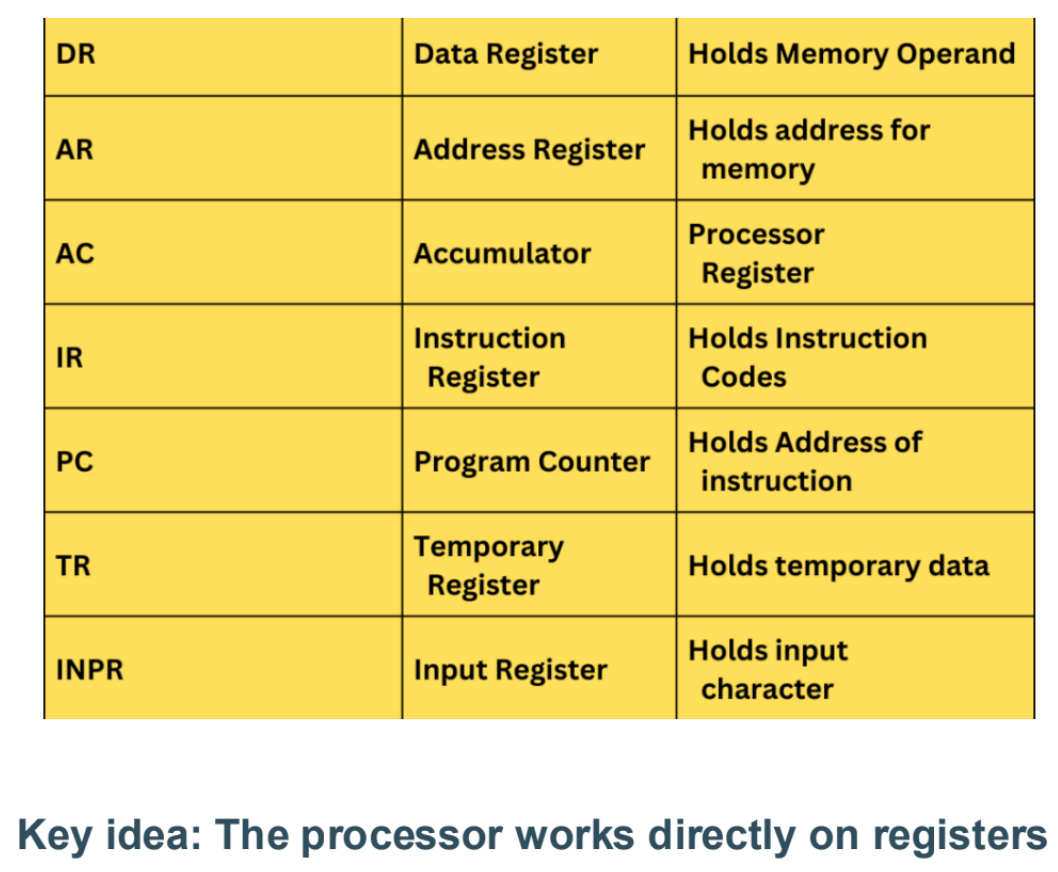
\includegraphics[width=0.6\textwidth]{soorten_registers.png}
  \caption{Soorten registers in een CPU}
  \label{fig:soorten_registers.png}
 \end{figure}
\subsubsection{Cache geheugen}
Cache functioneert als een brug tussen de supersnelle processor en het tragere RAM-geheugen. Het doel is om de traagheid van het RAM te verbergen door veelgebruikte data tijdelijk "dichtbij" te houden, het verminderd dus de tijd nodig om data op te halen van het RAM, dit is belangrijk voor de prestaties van de computer.
\newline
Het is fysiek kleiner dan ram, maar veel sneller, wel trager dan registers. Het is ook duurder dan RAM, dus er is een beperkte hoeveelheid cache geheugen in een computer.
\newline
De proff vergelijkt cache met een 'toolbelt' (gereedschapsgordel). Als je een programma draait met bijvoorbeeld een for- of while-loop, herkent het systeem dat bepaalde data constant opnieuw nodig is. Om tijd te besparen, wordt deze data tijdelijk in de cache bewaard in plaats van het telkens uit het tragere RAM te moeten halen.
\begin{figure}[H]
  \centering
  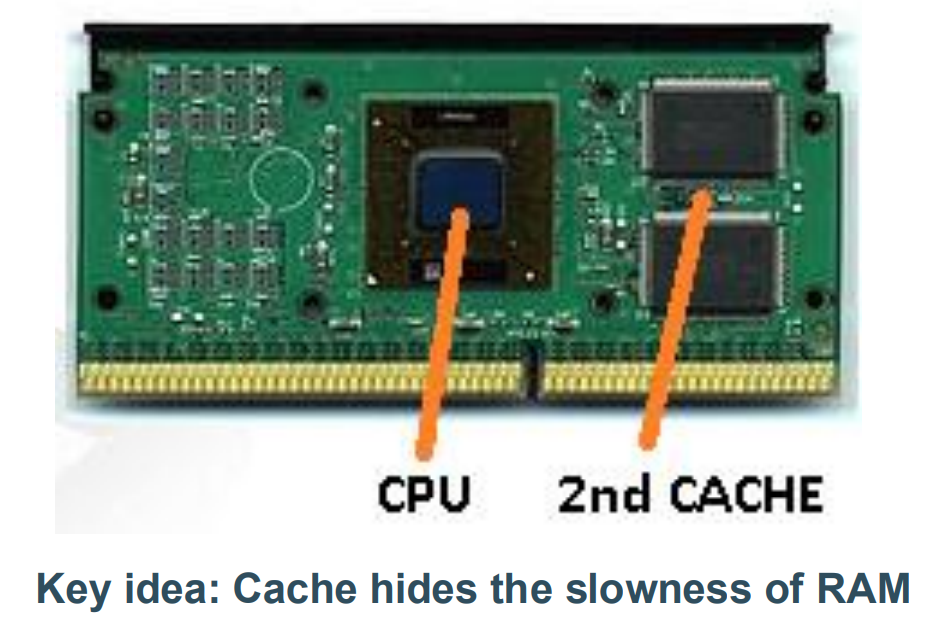
\includegraphics[width=0.5\textwidth]{cache.png}
  \caption{Cache}
  \label{fig:cache.png}
 \end{figure}
\subsubsection{RAM (Random Access Memory)}
Slaagt dus tijdelijk data en instructies op tijdens het uitvoeren van programma's. Het is dus trager dan cache en groter en het is volatiel. Dit is de grote "wachtkamer" of de werkplaats. Hier worden de actieve programma's, applicaties en grote datastructuren opgeslagen waar je op dat moment mee werkt. Hoe meer RAM je hebt, hoe meer zware programma's (of grote AI-modellen) je tegelijk open kunt houden.
\newline
\begin{conceptbox}[Waarom 'Random'?]
Dit wijst naar dat de data \textbf{niet sequentieel} wordt uitgelezen (zoals oudere opslagmethoden), vergelijk het met een video die je wilt afspelen, als je doorspoelt moet je eerst voorbij de eerdere stukken gaan. Bij ram hoeft dit niet, elk adress kan direct worden benaderd, dit maakt het veel sneller voor de CPU om toegang te krijgen tot de benodigde data.
\end{conceptbox}
\begin{figure}[H]
  \centering
  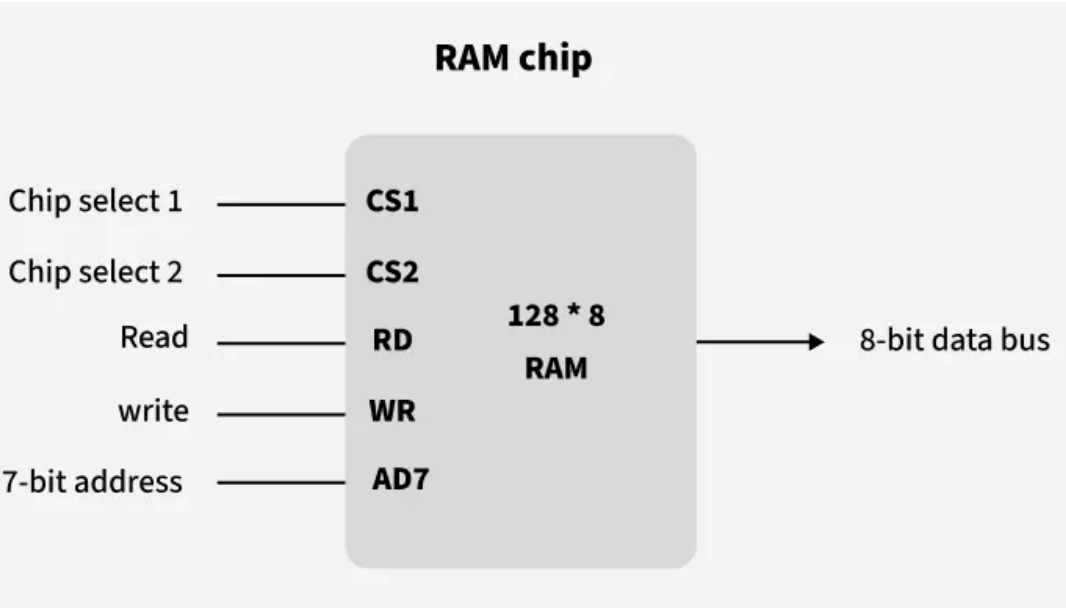
\includegraphics[width=0.6\textwidth]{ram.png}
  \caption{RAM}
  \label{fig:ram.png}
 \end{figure}
\newpage
\subsubsection{Secondary Memory}
Dit is de permanente opslag, zoals harde schijven of SSD's. Het is veel trager dan RAM, maar het is niet volatiel, dus het behoudt data zelfs als de computer is uitgeschakeld. Hier worden bestanden, programma's en het besturingssysteem opgeslagen.
\subsubsection{Alles te samen}
\begin{theorie}[Alles te samen]
 \begin{itemize}
        \item \textbf{Registers think:} De registers vormen de 'denkende' logica. Dit is de plek waar de processor op dat exacte moment zijn berekeningen uitvoert.
        \item \textbf{Cache remembers what you just used:} De cache onthoudt wat je zojuist hebt gebruikt. De professor voegt hier tijdens de les aan toe dat een moderne CPU-core vaak over meerdere lagen cache beschikt (Level 1, Level 2 en Level 3) om dit zo efficiënt mogelijk te doen.
        \item \textbf{RAM holds what you are working on:} Het RAM is je werkplaats. Het houdt de actieve programma's en data vast waar je op dit moment mee aan de slag bent.
        \item \textbf{Disk remembers everything:} De disk (zoals een HDD of SSD) is de langetermijnopslag die letterlijk 'alles onthoudt', en bewaart de data veilig voor later.
 \end{itemize}
\begin{figure}[H]
  \centering
  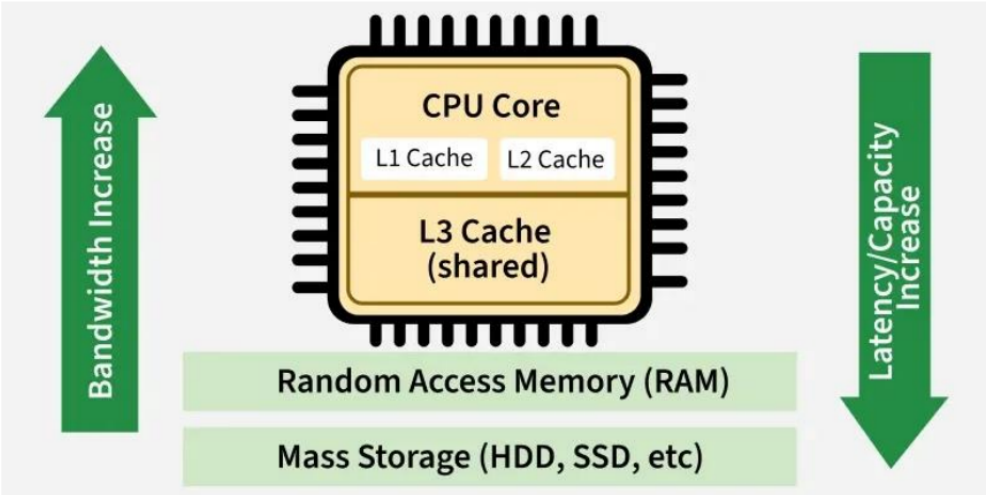
\includegraphics[width=0.8\textwidth]{allessamen.png}
  \caption{Alles te samen: Registers, Cache, RAM, Disk}
  \label{fig:allessamen.png}
\end{figure}
\end{theorie}
\newpage
\subsubsection{Memory hierarchy (geheugenhiërarchie)}
Een gestructureerde piramide die de keuzes en compromissen (trade-offs) in geheugen illustreert, het toont aan dat je niet tegelijkertijd supersnel, gigantisch groot én goedkoop geheugen kunt hebben.
\newline
Hoe hoger in de piramide, hoe dichter bij de processor, bandbreedte neemt toe, dus sneller maar de kosten stijgen dus en de capaciteit daalt.
\begin{figure}[H]
  \centering
  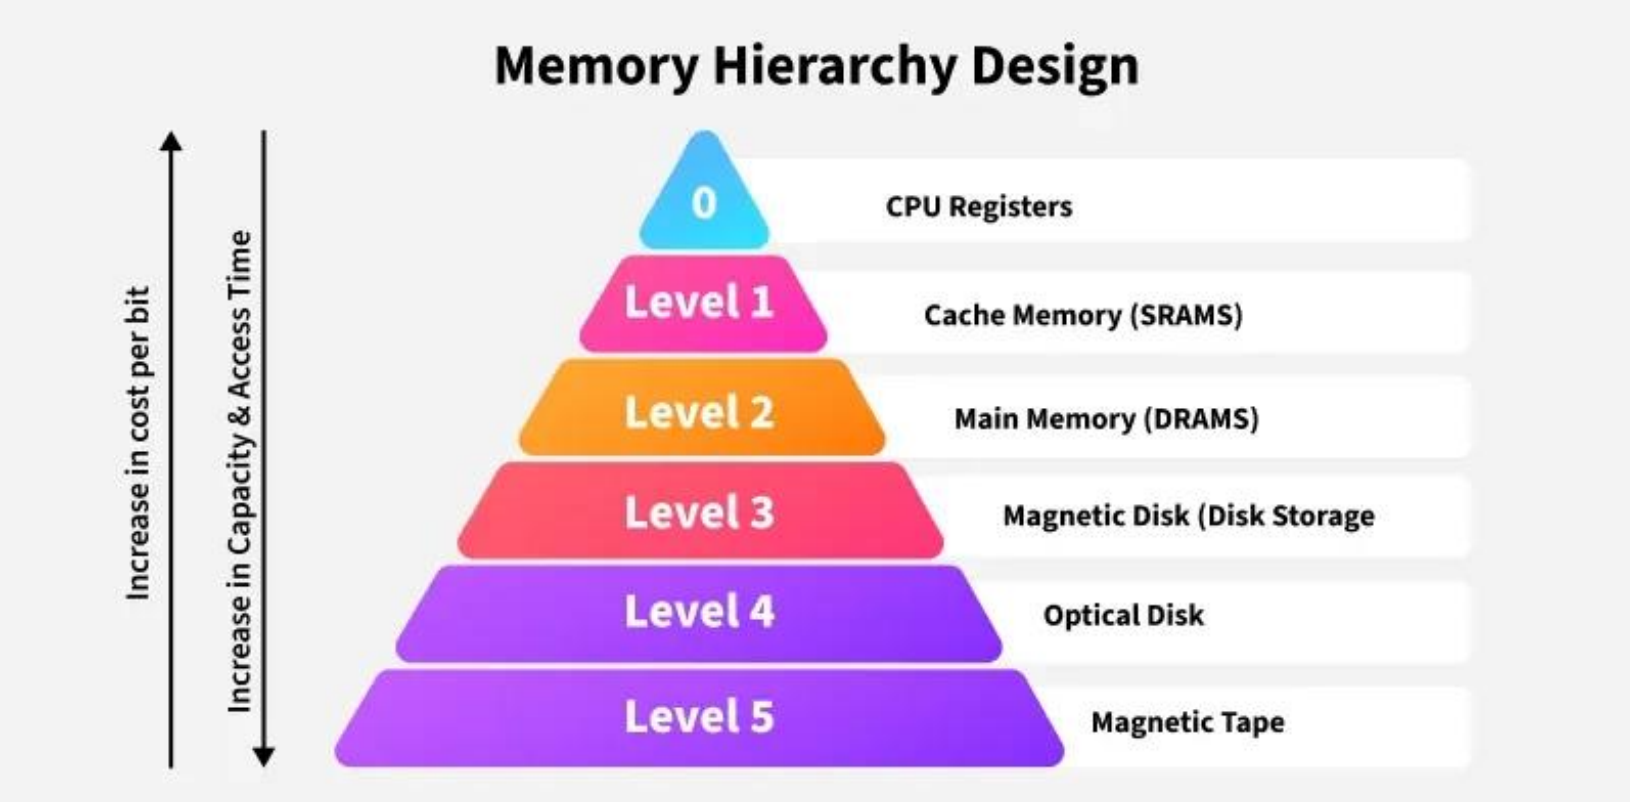
\includegraphics[width=0.8\textwidth]{memory_hierarchy.png}
  \caption{Geheugenhiërarchie}
  \label{fig:memory_hierarchy.png}
 \end{figure}
\subsubsection{Hoge integratie in moderne architectuur}
\begin{figure}[H]
  \centering
  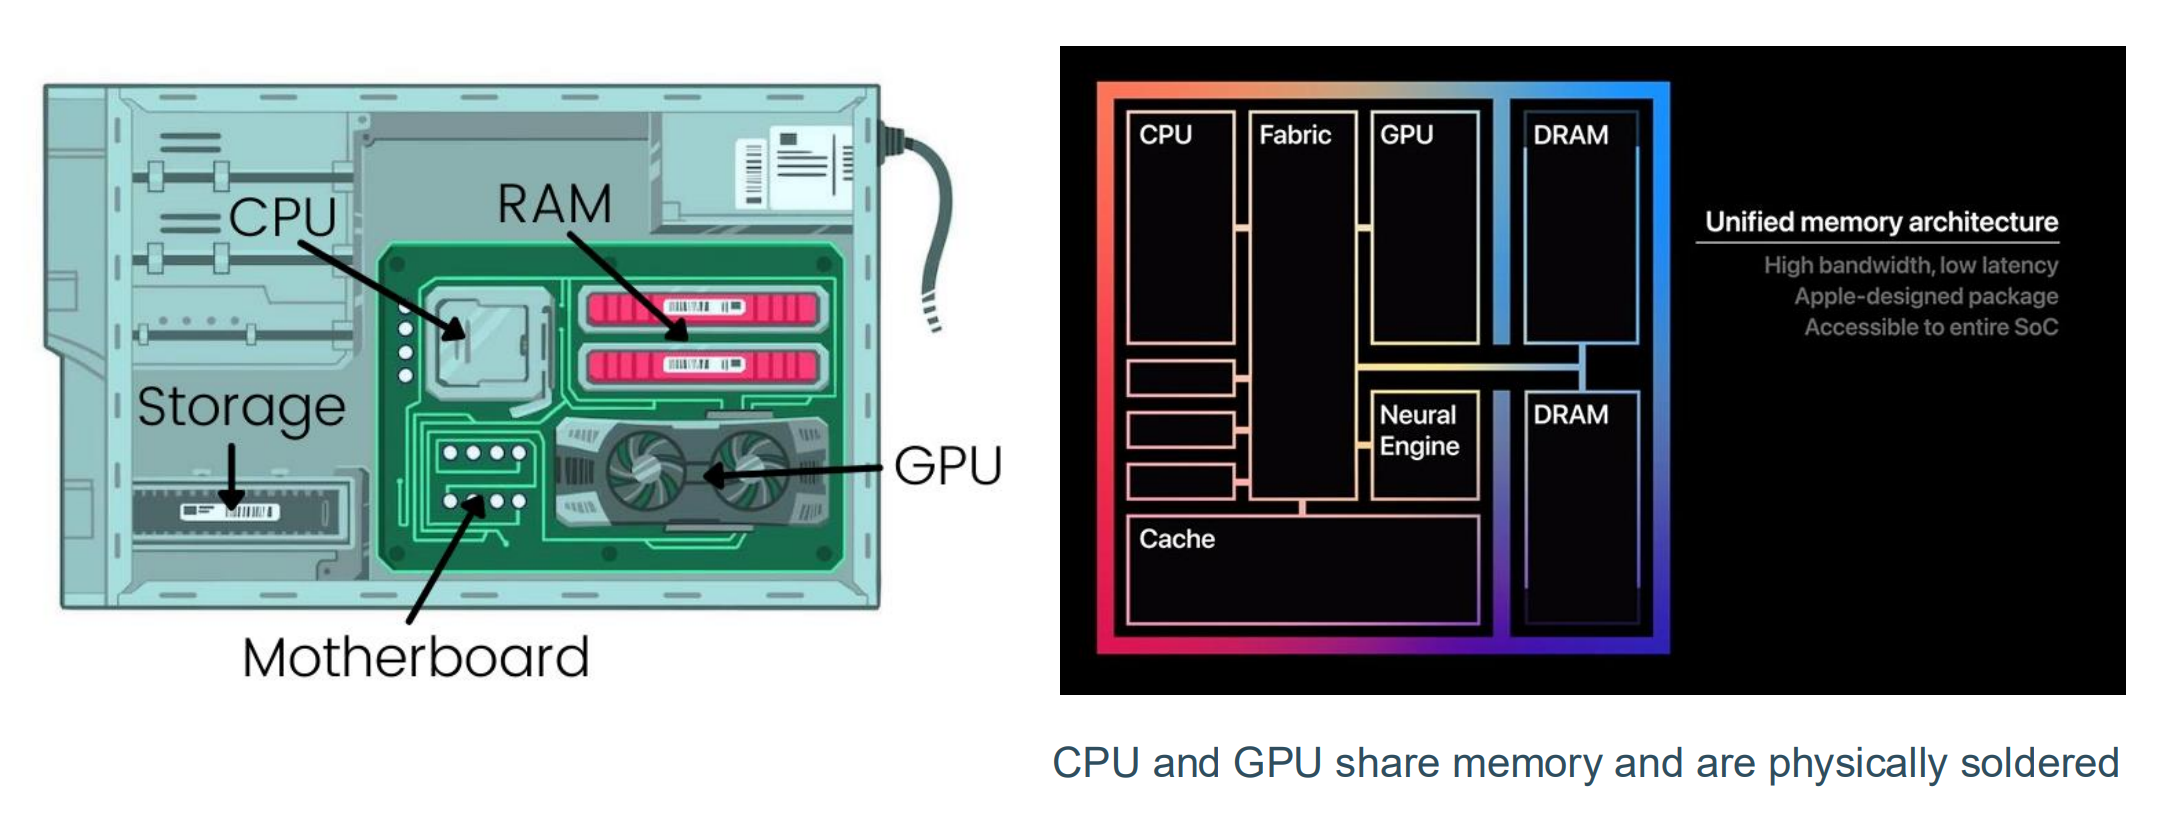
\includegraphics[width=0.8\textwidth]{modular_integrated.png}
  \caption{Klassiek modulair ontwerp vs moderne geïntegreerde architectuur}
  \label{fig:modular_integrated.png}
 \end{figure}
Op een klassiek moederbord zitten de CPU, de GPU en het RAM-geheugen als losse componenten in hun eigen aansluitingen. Dit is handig omdat je onderdelen kunt vervangen of upgraden, maar op de schaal van micro-elektronica zijn die componenten heel ver van elkaar verwijderd. De professor vergelijkt de fysieke afstand die data over zo'n moederbord moet afleggen met de afstand tussen 'Brussel en Shanghai'. Dit heen-en-weer sturen van data zorgt voor latency (vertraging) en kost veel extra stroom.
\newline
In een sterk geïntegreerde architectuur wordt alles samengebracht op één enkele chip (System on a Chip of SoC). De CPU, de GPU, de cache, de Neural Engine én het DRAM (werkgeheugen) delen fysiek dezelfde architectuur en zijn direct aan elkaar vastgesoldeerd
\newline
Omdat de onderdelen niet meer via 'lange' fysieke paden met elkaar hoeven te praten, is de dataoverdracht razendsnel en extreem energie-efficiënt, wat cruciaal is voor de batterijduur van mobiele apparaten.
\begin{conceptbox}[Memory Swap]
    De verbinding met de SSD is in deze systemen vaak zo snel, dat de computer de SSD bijna ongemerkt als tijdelijk werkgeheugen kan inzetten zodra het echte RAM vol dreigt te raken, dit concept heet \textbf{Memory Swap}.
\end{conceptbox}
\subsection{Computers}
We weten dus dat er verschillende soorten computers zijn, voor verschillende doelen(constraints), bvb: timing, energieverbruik, kost, vertrouwbaarheid, flexibiliteit, grootte, ...
\newline
Al deze 'constraints' leidden tot verschillende ontwerpen. Dus 'constraints drive architecture'(beperkingen sturen de architectuur).
\newline
Bij gsm's boeit latency op je whatsapp berichten bvb niet, wa boeit het als die 30ms later aankomen? Bij biotechnologische technologie (bvb een prosthesis) boeit dit natuurlijk wel.
\newline
Type computers die door ingenieurs gebruikt kunnen worden zijn de volgende :
\begin{itemize}
    \item \textbf{Embedded computers :} Dit zijn eigelijk microcontrollers zoals Raspberry PI of Arduino
    \item \textbf{Industrial computers :} Zoals SCALA of PLC
    \item \textbf{Consumer computers :} Wat je zelf thuis hebt zoals een laptop of desktop
\end{itemize}
\begin{figure}[H]
  \centering
  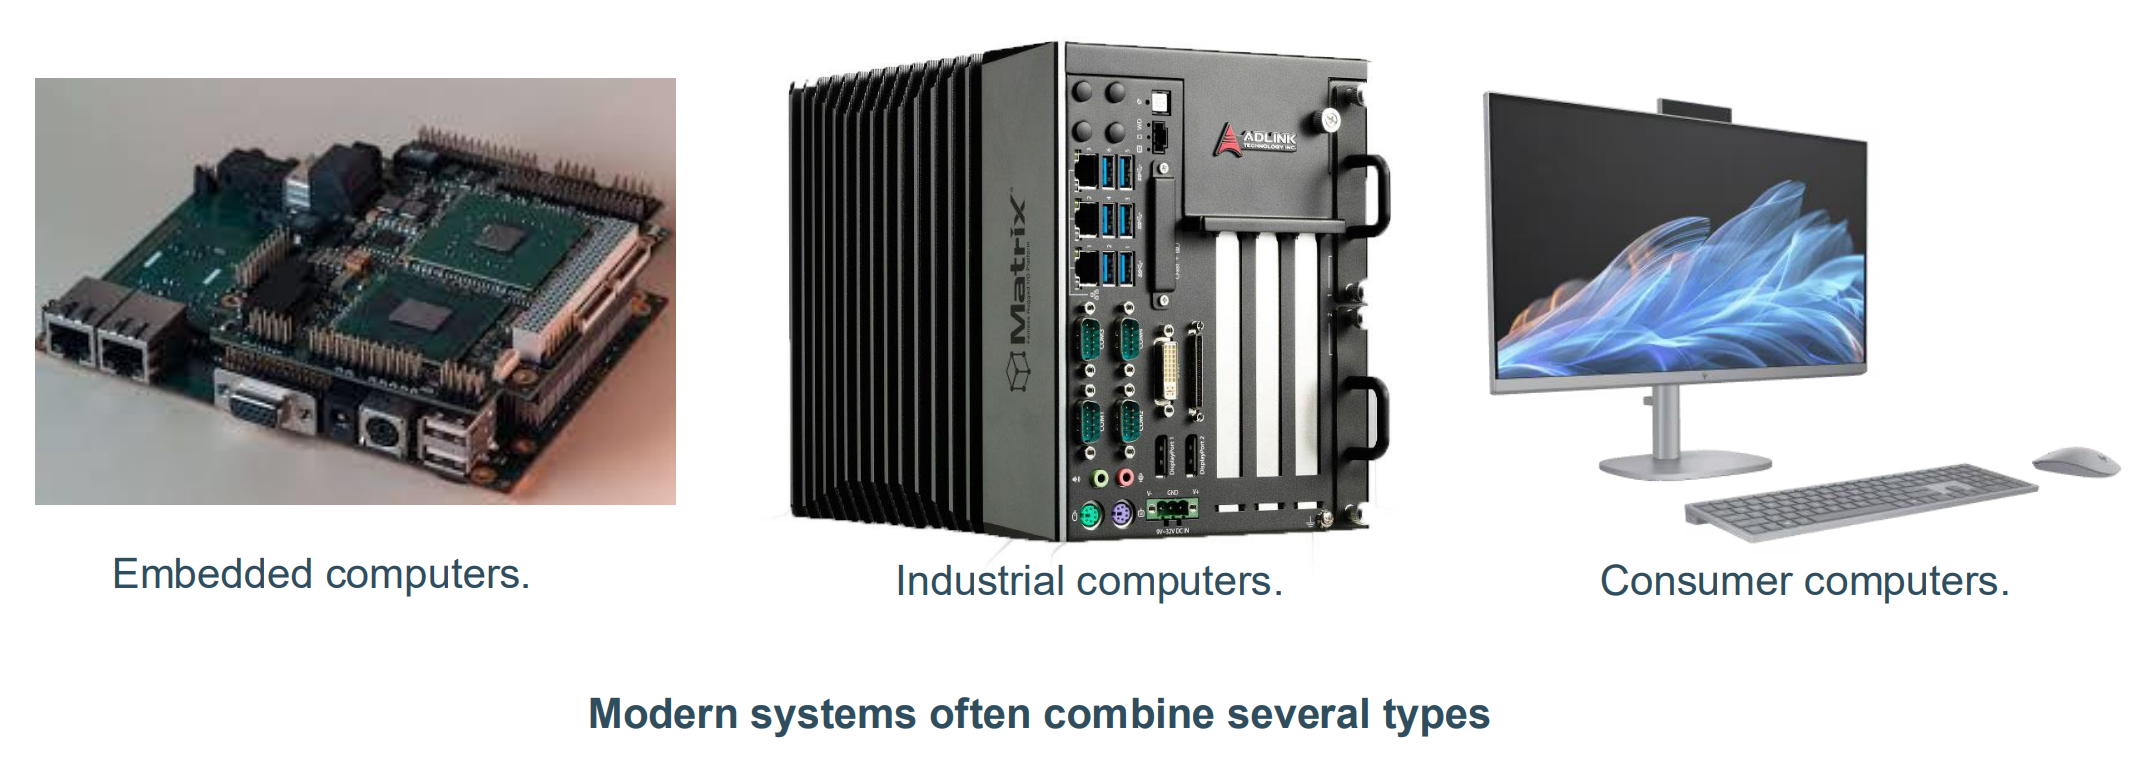
\includegraphics[width=0.8\textwidth]{typecomputers.png}
  \caption{Soorten Computers}
  \label{fig:typecomputers.png}
 \end{figure}
\subsubsection{Embedded computers}
Voorbeelden hiervan zijn dus : microcontrollers, motor controllers, automotive ECU's en Medische apparaten (want deze hebben lage latency).
\newline
In dit type computer kan je wel typisch niet multitasken ze hebben ook een gelimiteerd geheugen en opslag, ze hebben sterke constraints zoals 'real time'.
\begin{conceptbox}[Wat bedoelen ze met 'Real Time']
    Tijdens de les verduidelijkt de professor een veelvoorkomende misvatting hierover: 'real time' betekent niet simpelweg dat de computer heel erg snel is. Wat het wél betekent, is dat het systeem de absolute \textbf{garantie} kan geven dat een berekening of taak wordt afgerond \textbf{binnen een strikt gedefinieerd tijdvenster (time window)}. Het draait dus allemaal om voorspelbaarheid (determinisme).
\end{conceptbox}
\subsubsection{Industrial computers}

\end{document}